\chapter{Research Methodology}

Design science is a paradigm of real-world problem-solving by creating innovative artifacts. Therefore, Design science research tightly connected the IT artifact with the application domain. Furthermore, the need and desire to improve the current environment and methods motivate Design science research and therefore requires innovative artifacts to address such problems \cite{DSM_1}. The work adopted the research methodology of \cite{DSM_2} here and followed the research process model given in their work.

\section{Problem centered approach}
Although some work in the current field was done, this work aims to develop better tools to automatically extract the business process model for the broad audience of end users, i.e., users within a business organization with little knowledge about business process modeling or underlying technologies. Such motivation provides us with an opportunity to work on creating the tool mentioned above. This problem-centered approach leads us to the first step of the research process, according to \cite{DSM_2}.

\section{Problem Identification And Motivation}
Currently no automated approach exists that can create business process
visualizations from text in sufficient quality and generalizability

%Modeling business processes requires experts with relevant knowledge and can be exhausting and time-consuming. Thus, small companies usually cannot afford such experts and business managers usually prefer to describe processes using natural language. As a result, an organization usually process a large amount of text documents  \cite{literature_review_2}. However, the business process provides an intuitional overview of the business process and can potentially increase a company's productivity.

\section{Objectives of a solution}
Our objective is to create an easy-to-use tool that uses the Nature language processing technology to automatically extract information from organizations' texual documents and generate business process models.

\section{Design \& development}
The development of the new artifact adopted the critical success chain (CSC) method, which uses literature to support and consolidate the conceptual basis of the artifact designing \cite{DSM_2}. This work addressed the issues and the needs identified earlier, such as how to find a proper tool to extract information from texual documents or how to process such information to generate a BPMN model. The work conducted a literature review and used the helpful information from the selected papers to combine their ideas and develop our own artifact. The intended artifact is to develop a prototype that leverages the NLP technique to automatically extract business process models from texual documents.

\section{Demonstration}
In the demonstration activity, The work want to illustrate how can one use the proposed new artifact to solve instances of problem \cite{DSM_3}. The work will use the proposed artifact to convert the textual input into business process models where the users can quickly generate the BPMN models even though they have no knowledge of process modeling. We will run simulations to support our approach and to prove that our approach can minimize the workload of business process modeling.

\begin{figure}[h]
    \centering
    \caption{Design Science Research Process}
    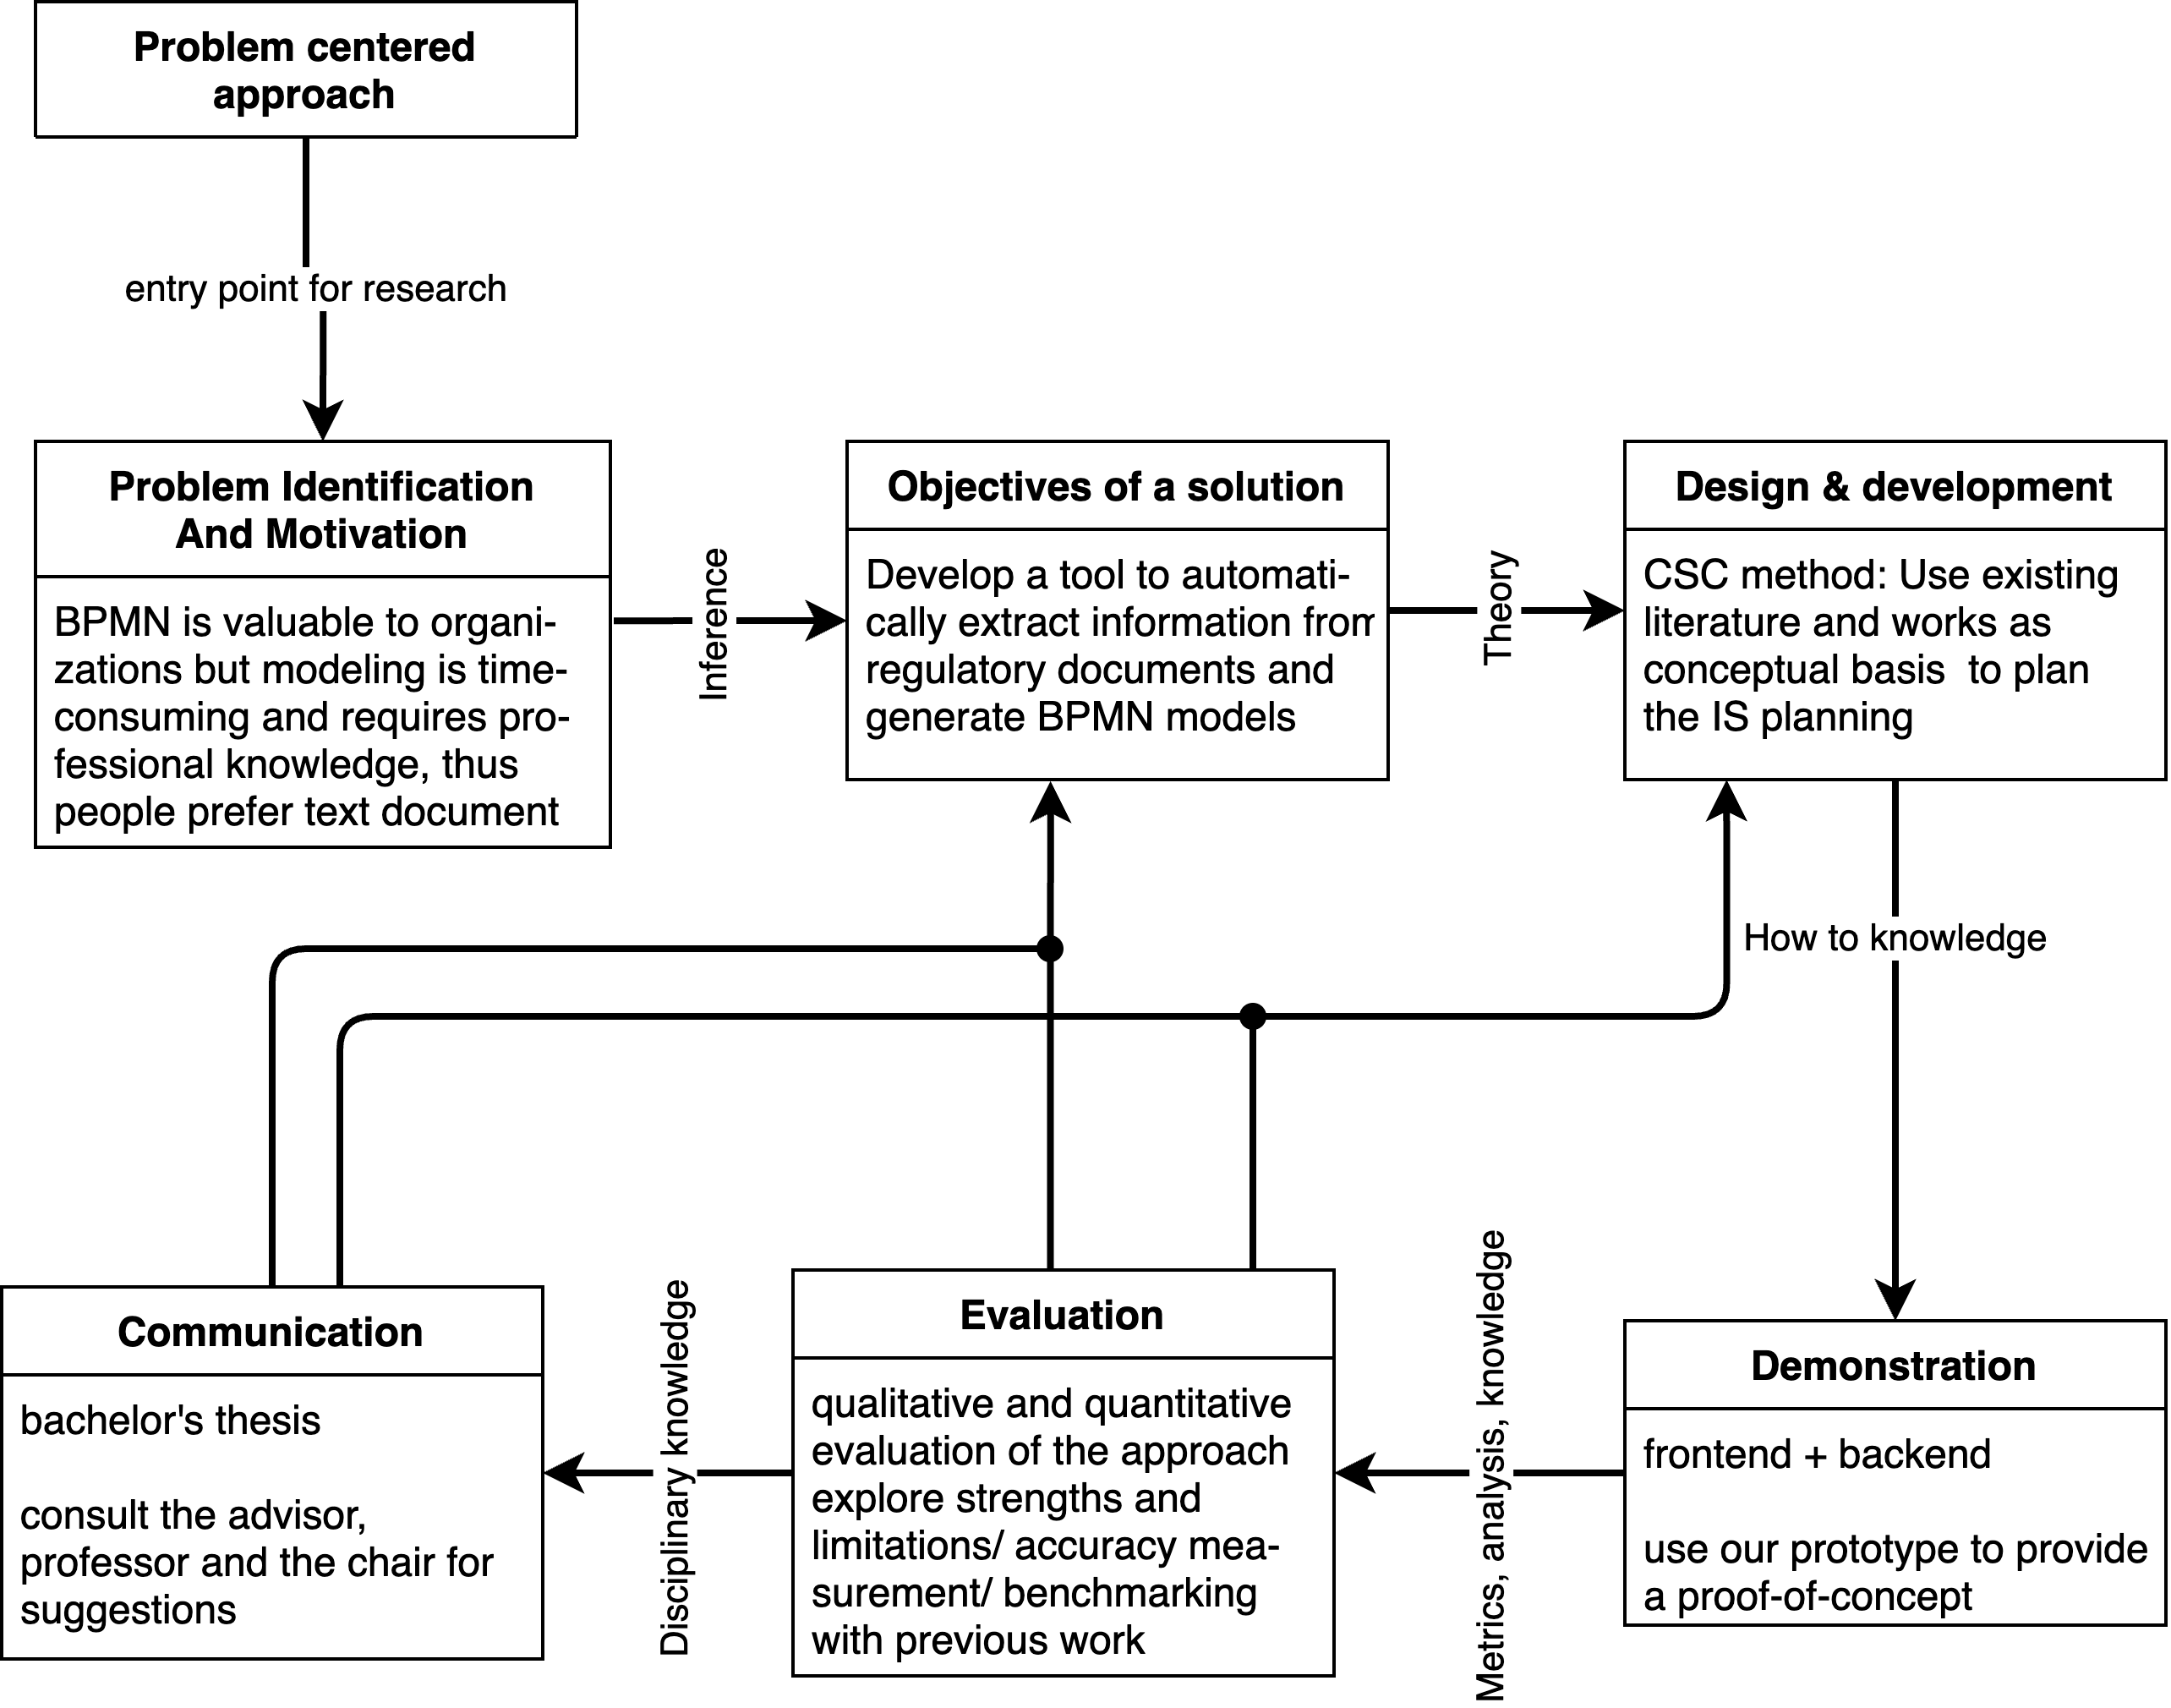
\includegraphics[width=0.9\textwidth]{tum-resources/images/DSM.png}
    \floatfoot{Overview of the research and artifact design steps for research methodology}
\end{figure}

\section{Evaluation}
The evaluation phase is vital in the design of an artifact. The evaluation examines how well the designed artifact solves the problem, which involves comparing the actual output of the problem and the output generated by the artifact \cite{DSM_3}. The evaluation is divided into qualitative and quantitative parts. In the qualitative evaluation, The strengths and limitations of the approach are explored, and we will communicate with the BPMN modeling experts to check the model compliance of our generated BPMN model. In quantitative evaluation, The accuracy of the approach will be numerically identified. The work intended to first manually generate business process models using several different kinds of documents. In the next step, the same documents will be used by the artifact to automatically generate BPMN models. Then the similarity of these two models will be computed and compared to determine the quality of the artifact. \cite{t2m_1} suggests that the metric of \textit{Graph Edit Distance} can be leveraged to achieve such goal. Another aspect of the quantitative aspect is to benchmark the proposed approach with the previous work. The work will look into the approach's accuracy and program execution time compared to the previous work. Based on the evaluation results, we will decide whether to iterate back the step three to modify and improve the artifact if the outcome is not very promising or to continue to the communication phase. Further improvement is also possible to be left to the subsequent projects.

\section{Communication}
To ensure the delivery of the desired artifact, every aspect of the problem and the design of the artifact will be communicated and discussed with the relevant stakeholders \cite{DSM_3}. Since this is a bachelor's thesis, the primary contact is the author's advisor. Furthermore, the work will also seek advice and suggestions from Prof. Dr. Stefanie Rinderle-Ma and the corresponding Chair of Information Systems and Business Process Management (i17). 




